 %██████╗██╗   ██╗██████╗ ██╗   ██╗███████╗    ███████╗██╗████████╗████████╗██╗███╗   ██╗ ██████╗ 
%██╔════╝██║   ██║██╔══██╗██║   ██║██╔════╝    ██╔════╝██║╚══██╔══╝╚══██╔══╝██║████╗  ██║██╔════╝ 
%██║     ██║   ██║██████╔╝██║   ██║█████╗      █████╗  ██║   ██║      ██║   ██║██╔██╗ ██║██║  ███╗
%██║     ██║   ██║██╔══██╗╚██╗ ██╔╝██╔══╝      ██╔══╝  ██║   ██║      ██║   ██║██║╚██╗██║██║   ██║
%╚██████╗╚██████╔╝██║  ██║ ╚████╔╝ ███████╗    ██║     ██║   ██║      ██║   ██║██║ ╚████║╚██████╔╝
 %╚═════╝ ╚═════╝ ╚═╝  ╚═╝  ╚═══╝  ╚══════╝    ╚═╝     ╚═╝   ╚═╝      ╚═╝   ╚═╝╚═╝  ╚═══╝ ╚═════╝ 
%.:..:..:..:..:..:..:..:..:..:..:..:..:..:..:..:..:..:..:..:.
\section{Curve Fitting}

\subsection{Gaussian Channel Model}
The equation representing BER for the project's OFDM variant in a Gaussian channel is:
\begin{align}
	y = f(x) &=
	\begin{cases}
		0.47Q \left(\frac{x - 7.5}{2.5}\right) & -\infty \leq x \leq 9.5 \\
		0.15Q \left(\frac{x - 10.5}{1.17}\right) & 9.5 < x \leq 15 \\
		0 & \text{otherwise}
	\end{cases}
\end{align}
\begin{figure}[htpb!]
    \centering
    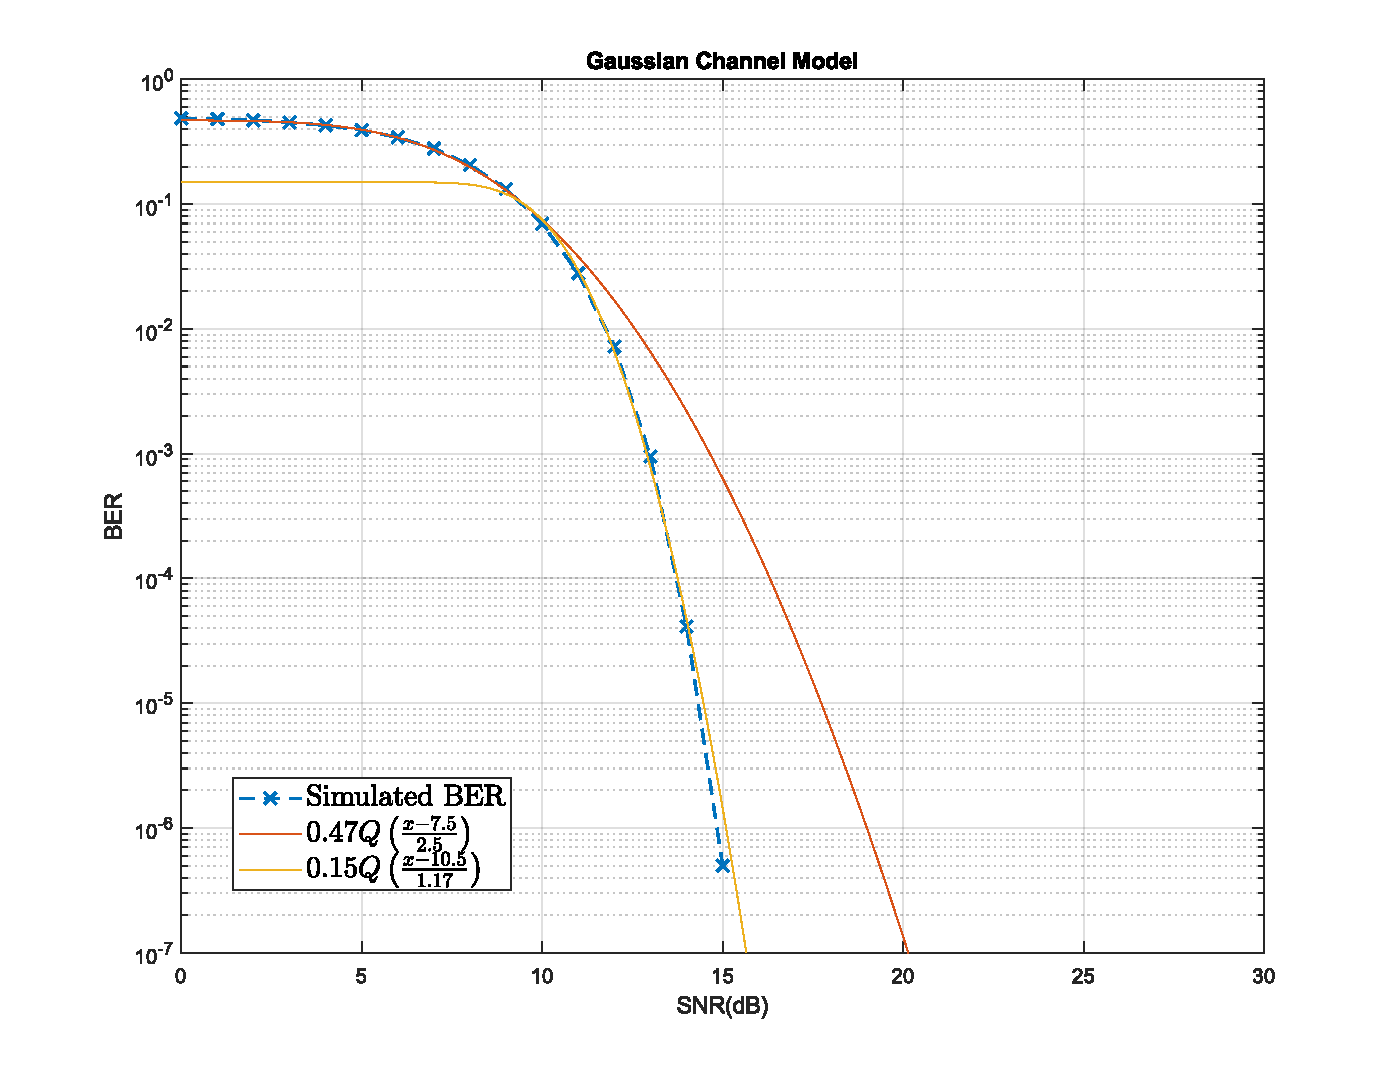
\includegraphics[scale=0.6]{Graphics/Methodology/GaussCurveFit.pdf}
    \caption{AWGN Channel curve fitting}
    \label{fig:gaussCurveFit}
\end{figure}
\pagebreak

\subsection{Rayleigh Channel Model}
The equation representing BER for the project's OFDM variant in a Rayleigh fading channel is:
\begin{align}
	y = f(x) &=
	\begin{cases}
		0.5Q \left(\frac{x - 11.1}{3.05}\right) & -\infty \leq x \leq 17 \\
		1_E4Q \left(\frac{x - 35}{11}\right) & \text{otherwise} \\
	\end{cases}
\end{align}
\begin{figure}[htpb!]
    \centering
    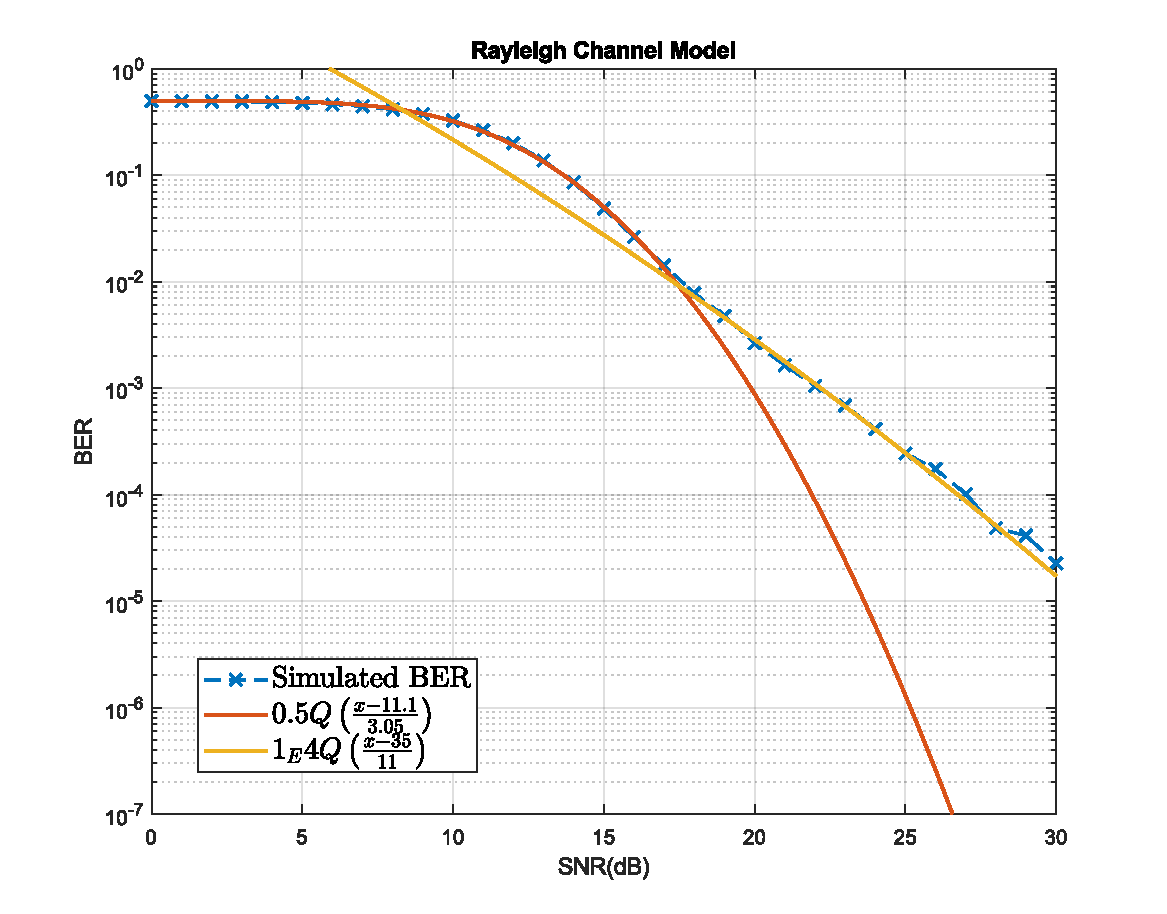
\includegraphics[scale=0.6]{Graphics/Methodology/RaylCurveFit.pdf}
    \caption{Rayleigh Channel Curve Fitting}
	\label{fig:raylCurveFit}
\end{figure}
\pagebreak

\subsection{Rician Channel Model}
The equation representing BER for the project's OFDM variant in a Rician fading channel is:
\begin{align}
	\label{res:RiceFn}
	y = f(x) &=
	\begin{cases}
		0.5 & -\infty < x \leq 0 \\
		aQ \left(\frac{x - b}{c}\right) & 0 < x \\
	\end{cases}
\end{align}
\begin{mathDef}
	\mathSymb{x}{\gls{SNR}}
\end{mathDef}
The values of \(a\), \(b\) and \(c\) are determined by \(K\) according to equations \eqref{eq:meth:a}, \eqref{eq:meth:b} and \eqref{eq:meth:c} respectively.
The range of \(K\) for which equation \eqref{res:RiceFn} is valid is:
\begin{equation}
	0 \leq K \leq 10.5
\end{equation}
\begin{figure}[htpb!]
    \centering
    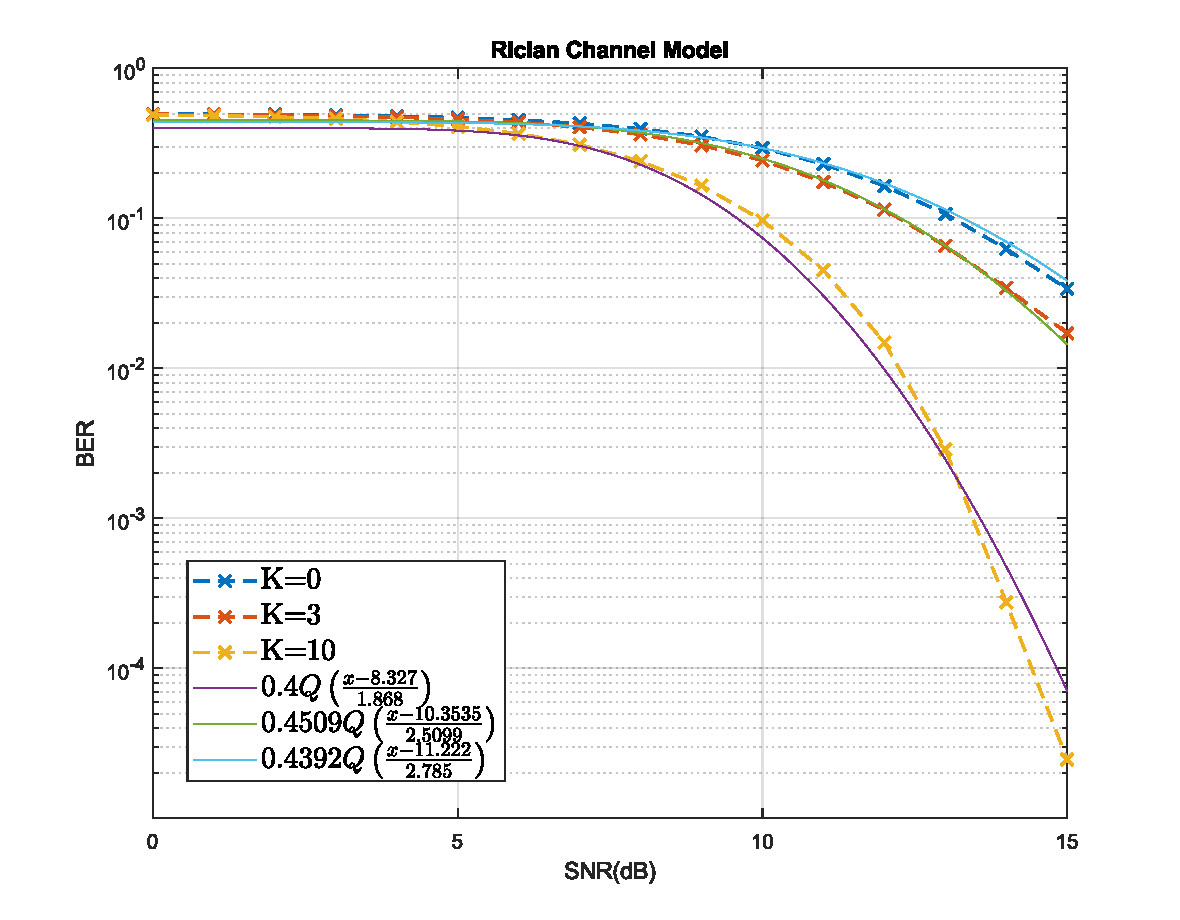
\includegraphics[scale=0.56]{Graphics/Methodology/RiceCurveFit.pdf}
    \caption{Rician Channel Curve Fitting}
	\label{fig:riceCurveFit}
\end{figure}


\pagebreak


